\chapter{$S$-Duality and Line Defects in the Twisted 4D Theory\label{ch:finale}}

The aim of this chapter is to first develop for the reader a picture of $\mathcal N = 4$ Supersymmetric Yang-Mills (SYM) theory together with its topological twists. With this, we bring together the ideas of the previous chapters and study the actions of line defects on the categories of boundary conditions of two topological twists of $\mathcal N=4$ SYM.

	Since geometric Langlands associates to each 2D complex curve an equivalence of categories, and since TQFT associates a category to each codimension two submanifold, following a blurb of Witten in \cite{witten2017}, the reason that the Langlands correspondence is realized by a duality of a gauge theory in four dimensions is that $2+2=4$. Moreover, a quick mathematical calculation gives that $4-1 = 3$. Taking one dimension to be ``time'', we will see that the line operators of the 4D theory can be viewed as acting like point insertions of singularities along a given 3-manifold $W$. This is where the Bogomolny equations of the prior chapter shall enter into the picture, and we will make a connection of the solution of the Bogomolny equations to the space of Hecke modifications.

\section{Setting the Stage} % (fold)
\label{sec:setting_the_stage}

\subsection{Reduction from Ten Dimensions} % (fold)
\label{sub:reduction_from_ten_dimensions}

One of the simplest ways to arrive at 4D $\mathcal N=4$ SYM is to begin with supersymmetric gauge theory on $\rr^{10}$ with gauge group $G$ \cite{kapustin2006}. Throughout this chapter, we will be working in \emph{Euclidean signature}. Recalling from Section \ref{sub:spin_representations}, $\Spin(10)$ is known to have two inequivalent spin representations $S^+$ and $S^-$, our supersymmetry will be of the form $\mathcal N = (1, 1)$. In the 10D theory, we have two fields, $A$ and $\lambda$. $A$ is a connection on a principal $G$-bundle $P$ while $\lambda$ transforms as a positive chirality spinor with values in the adjoint representation\footnote{There will also be a negative chirality spinor $\overline \lambda$, but it will not play an important role in what is to come.}, namely we consider sections $\lambda \in \Gamma(M, S^+ \otimes \ad P)$. We have $F = \dd_{A} A$.

``Bosonic'' will be taken to mean terms consisting of only the connection $A_{10D}$ and its derivatives. ``Fermionic'' will be taken to mean terms involving a the spinor $\lambda$. This is standard convention in any textbook on quantum field theory, see for example \cite{schwartz2014}. This theory has $16$ supercharges $Q_a$ transforming in the $S^-$ representation.

% The generator of supersymmetry is a spinor in $S^+$. This theory has $16$ supercharges $Q_a$. The \emph{supersymmetric variation} of the fields is given by:
% \[
% \begin{aligned}
% 	\sum_a [\epsilon^a Q_a, {A_{10D}}_I] &= i \overline \epsilon \Gamma_I \lambda\\
% 	\sum_a [\epsilon^a Q_a, \lambda] &= \Gamma^{IJ} {F_{10D}}_{IJ} \epsilon
% \end{aligned}
% \]
The action here is:
\begin{equation}
	S = \frac{1}{e^2} \int \tr \left(F_{10D} \wedge \star F_{10D} - i \overline \lambda \Gamma \dd_A \lambda \right).
\end{equation}
where $\Gamma$ is the chirality operator discussed in Section \ref{sub:lie_superalgebras}.

The reduction to 4 dimensions is done in a similar manner to how we proceeded in Chapter~\ref{ch:monopoles}. Namely, we assume all fields are independent of the last six direction. This gives us a new connection which we will again denote by $A =A_\mu d^\mu$ in 4D together with six scalar fields $\phi_i$. The curvature $F$ decomposes into three terms. The first is the curvature in 4D, which we will again denote by $F$, the second consists of covariant derivatives of the $\phi_i$, $\dd_A \phi_i$, and the last consists of commutators $[\phi_i, \phi_j]$. All together, the bosonic part of the action can be written as:
\begin{equation}
	\frac{1}{e^2} \int_M \tr\left( F \wedge \star F + \sum_i \dd_A \phi \wedge \star (\dd_A \phi) +  \sum_{i < j} [\phi_i, \phi_j]^2 \mathrm{Vol}_M \right)
\end{equation}
The fermionic part can be similarly decomposed into four spinors $\lambda^a$ transforming in $\ad(E) \otimes S^+$ and four spinors $\overline \lambda_a$ transforming in $\ad(E) \otimes S^-$. In Minkowski signature $\lambda$ and $\overline \lambda$ are conjugates but in Euclidean signature they are independent \cite{kapustin2008}.

The reduced 4D theory gains an $\mathrm{Spin}(6)$ symmetry acting on the fields which is in fact the $R$ symmetry group from Section~\ref{sec:supersymmetry}. The scalar fields $\phi_i$ transform in the vector representation of this group, while the $\lambda$ and $\overline \lambda$ transform as spinors and dual spinors of this group as well.

% \begin{equation}
% 	S = \frac{1}{e^2} \int dx^4 \tr\left( \frac{1}{2} F_{\mu \nu} F^{\mu \nu} + \sum_i D_\mu \phi^i D^\mu \phi_i + \frac12 \sum_{i,j} [\phi_i, \phi_j]^2 \right)
% \end{equation}
On $M=\rr^4$ the 16 supersymmetries will transform as $\mathcal N=4$ copies of the 4-dimensional spin representation of $\Spin(4)$. We will have $\overline Q^A_{\alpha}$ and $Q^A_{\dot \alpha}$ for $A \in \{1,2,3,4\}$ and $\alpha, \dot \alpha \in \{1,2\}$ transforming as spinors and dual spinors in $\mathrm{Spin}(6)$ and also as spinors and dual spinors for the spacetime structure group $\mathrm{Spin}(4)$.


\begin{phys}
	$\mathcal N=4$ Super-Yang Mills theory is the unique field theory of maximal supersymmetry in four dimensions.
\end{phys}

Further, this theory is \emph{scale invariant}. By the usual arguments \cite{schwartz2014}, it is easy to see that the mass dimension of the coupling constant $e$ must be 0, though it is much harder to see that renormalization will not contribute a mass scale. Scale invariance, together with the Poincar\'e symmetry of $\rr^4$ combine in this case to form a \emph{conformally invariant} theory known as a \textbf{conformal field theory}. For an exposition on conformal field theory in dimensions greater than two, see \cite{simmons2016}. This conformal invariance will be \emph{crucial} for the necessary duality to make sense, as otherwise the nontrivial renormalization flow would violate the Montonen-Olive duality between electric and magnetic charge, to be introduced in the next subsection and summarized in depth in section three of \cite{kapustin2008}.


There is also a parameter $\frac{i \theta}{8\pi} \int_M \tr (F \wedge F)$ that can be added to the action where $\theta$ is called the \textbf{instanton angle}. By the usual Chern theory arguments (see Section~\ref{sub:the_instanton_number}), this depend only on the topology of the principal $G$-bundle of the gauge theory.
\begin{obs}
	The theory is invariant under $\theta \to \theta + 1$.
\end{obs}
\begin{proof}
	Since $\frac{1}{8\pi} \int_M \tr (F \wedge F)$ is an integer, the path integral is
	\[
		\mathcal Z = \sum_{\substack{P \\ \text{principal bundles}}} \int \mathcal D\{ Fields \} \, e^{- S_E[\Phi]}.
	\]
	For $\theta \to \theta+1$ we get an additional factor of 
	\[
		e^{i \int_M \tr(F \wedge F)}
	\] 
	to the action. Since the instanton number is an integer by the same arguments as in Chapter~\ref{ch:instantons}, this will have no effect on any of the observables of the theory.
\end{proof}

In general $e^2$ and $\theta$ are two parameters determining the coupling properties of the theory, and are more generally bundled together into a single coupling constant $\tau = \theta/2\pi + 4\pi i/e^2$. We have just seen that $\tau \to \tau+1$ is a symmetry of the theory. Next, we will discuss a far less trivial symmetry. 

% subsection reduction_from_ten_dimensions (end)

\subsection{Montonen-Olive Duality} % (fold)
\label{sub:montonen_olive_duality}

	For this entire chapter, we will take $G$ is a simple Lie group that is not in the $B$ or $C$ series. The \textbf{lacing number} $n_{\gg}$ of $G$ is defined to be $3$ for the group $G_2$, $2$ for the groups $F_4$, and $1$ otherwise. There are also arguments for treating the $B$ and $C$ series (see section 2.2 of \cite{kapustin2006}), equivalently giving them lacing number $2$.

	In physics, a duality between a theory with coupling constant $e$ and coupling constant $1/e$ is called a \emph{strong-weak} duality, more generally known as \textbf{\emph{S}-duality}. What is special about $\mathcal N=4$ super Yang-Mills theory is that it is conjectured to exhibit a strong-weak duality in the coupling constant $\tau$. 
	

	\begin{concept}[Montonen-Olive Duality]
		In 4D $\mathcal N = 4$ supersymmetric Yang-Mills theory with gauge group $G$ and complex coupling constant $\tau$, any correlator of observables
		\[
			\left< \mathcal O_1 \dots \mathcal O_n \right>_{\tau, G} := \int \mathcal{D}\{ Fields \}\, \mathcal O_1 \dots \mathcal O_n \, e^{-S}
		\]
		can be rewritten in terms of Yang-Mills theory with inverse coupling constant $-1/n_{\gg} \tau$ on the Langlands dual group $\check G$ as a correlator of dual operators $\tilde {\mathcal O_1} \dots \tilde {\mathcal O_n}$
		\[
			\left< \mathcal O_1 \dots \mathcal O_n \right>_{\tau, G} = \left< \tilde{\mathcal O_1} \dots \mathcal O_n \right>_{-1/n_\gg \tau, \check G}.
		\]
	\end{concept}
	
	Thus, in a given theory with coupling constant $\tau = \theta/2\pi + 4\pi i/e^2$, we have two symmetries $\tau \to \tau+1$ and $\tau \to -1/\tau$ (in the simply laced case), which we know generate the larger set of transformations:
	\[
		\tau \to \frac{a \tau + b}{c \tau + d}.
	\]
	This is $\SL(2, \zz)$.
	
	This duality was first noted by Goddard, Montonen, Olive, and Nuyts in \cite{montonen1977, goddard1977}, as an observation between the duality of magnetic charge . It does not seem to be able to be made compatible , but there is strong evidence that $\mathcal N=4$ super Yang-Mills theory exhibits this duality. From here forward, we will \emph{assume} the existence of this duality (often abbreviated as GNO or MO duality), and derive constructions related to the Langlands conjecture, in particular the geometric Satake equivalence. 
	
	We are in a place where we should at least give a rough characterization of the Langlands dual group. Rather than giving the explicit definition, we simply characterize the property that will be useful to us.
	\begin{fact}[Langlands Dual Group]
		Let $G$ be a reductive group. The coweight lattice of $G$ is the same as the weight lattice of its Langlands dual $\check G$. Consequently, for $G$ a real compact group, let $T$ be a maximal torus in $G$. There is a corresponding maximal torus $T^\vee$ in $\check G$ so that
		\[
			\mathrm{Hom}(U(1), T) \cong \mathrm{Hom}(T^\vee, U(1)).
		\]
	\end{fact}
	This fact will be sufficient to guide us in the constructions relevant to the rest of this chapter.
	
% subsection montonen_olive_duality (end)

\subsection{Topological Twisting} % (fold)
\label{sub:topological_twisting}

	In this subsection we aim to give the reader a basic understanding of the process of topological twisting, and how this changes a field theory. Recall, from \ref{sec:supersymmetry} the following:
	\begin{phys}[Sector]
		Given a supersymmetry operator $Q$ such that $Q^2 = \frac{1}{2} [Q, Q] = 0$, we define the sector of our theory $\mathcal E$ by the set of $Q$ invariants, and denote this as $(\mathcal E, [Q, -])$.
		
		Slightly more precisely, $[Q, -]$ defines a differential operator, and the ``observables'' become exactly those gauge-invariant quantities annihilated by $Q$ modulo those that are $Q$-exact.
	\end{phys}
	
	
	\begin{phys}[Topological Twist]
		Given a supersymmetric (SUSY) field theory $\mathcal E$, a topological twist is a procedure for extracting a sector of $\mathcal E$ that depends only on the topology of the spacetime manifold. The resulting field theory is \textbf{topological} in the definition of Section~\ref{sec:topological_quantum_field_theory}
	\end{phys}
	In general this involves a homomorphism from the universal cover of the structure group of the spacetime tangent space $TM$ to the R-symmetry group. For our four-dimensional $\mathcal N = 4$ case this is
	$$\rho : \mathrm{Spin}(4) \to \mathrm{Spin}(6).$$
	This redefines how the fields transform under the cover of the Lorentz group, $\mathrm{Spin}(4)$. 
	
	The twist that will give us the geometric Langlands duality comes from considering first the following equivalence-class of obvious embeddings.
	$$\mathrm{Spin}(4)/\zz_2 = \SO(4) \hookrightarrow \SO(6) = \mathrm{Spin}(6)/\zz_2$$
	given by:
	\[
		\begin{pmatrix}
			* & * & * & * & 0 & 0 \\
			* & * & * & * & 0 & 0 \\
			* & * & * & * & 0 & 0 \\
			* & * & * & * & 0 & 0 \\
			0 & 0 & 0 & 0 & 1 & 0 \\
			0 & 0 & 0 & 0 & 0 & 1
		\end{pmatrix}.
	\]
	This embedding will then have a $\zz_2$ lift giving our desired $\rho$. 
	
	Another way to get this embedding is to note that by the accidental isomorphisms, $\mathrm{Spin}(6) \cong \SU(4)$ and $\mathrm{Spin}(4) \cong \SU(2)_L \times \SU(2)_R$, which embeds block-diagonally into $\SU(4)$ as
	\[
		\begin{pmatrix}
			\SU(2)_L & 0 \\
			0 & \SU(2)_R
		\end{pmatrix}.
	\]
	
	After twisting by $\rho$, the group $\mathrm{Spin}(4)$ acts differently on the supersymmetry generators. In particular, of the 16 generators, one of the left-handed and one of the right-handed supersymmetries become scalars under the new action of $\mathrm{Spin}(4)$. We thus get scalars $Q_l, Q_r$, and any (complex) linear combination of these gives rise to a different ``sector'' of invariants\footnote{For a more detailed overview of what is meant by this language, the reader is invited to consult a textbook on quantum field theory discussing the BRST quantization scheme. The notes of \cite{van2005aspects} and Weinberg's second volume on quantum field theory \cite{weinberg1995quantum} are good resources for this}. Clearly overall scaling does not matter in defining the invariant fields, so we have $\mathbb P^1 (\mathbb C)$ of subsectors to chose from.
	
	Upon a choice of $Q = u Q_l + v Q_r$, after some manipulation, one can rewrite the $\mathcal N=4$ Yang-Mills action as:
	\begin{equation}
		S = \{ Q , V \} + \frac{i \theta}{8\pi^2} \int_M \tr(F \wedge F) - \frac{1}{e^2} \frac{v^2-u^2}{v^2+u^2} \int_M \tr (F \wedge F).
	\end{equation}
	Here $V$ is some relatively complicated gauge invariant function of the fields that will not matter for the observables in the BRST-quantized theory, since it contributes a $Q$-exact term. Note that though there is metric dependence in $V$, the remaining terms involve only $\int_M \tr (F \wedge F)$, which we know to be metric independent, depending only on the topology of the principal bundle. 
	
	\begin{fact}
		Any such sector obtained by a choice of $Q$ defines a theory that is independent of the Riemannian metric (i.e. diffeomorphism invariant). Further, this topological theory can be defined on a general curved four-manifold $M$.
	\end{fact}
	
	In general, we can bundle $\frac{\theta}{2\pi} +  \frac{v^2-u^2}{v^2+u^2} \frac{4\pi i}{e^2}$ into a single parameter $\Psi$ known as the ``canonical parameter'' by Kapustin and Witten \cite{kapustin2006} and write:
	\[
		S = \{ Q, V\} + \frac{i \Psi}{4\pi} \int_M \tr (F \wedge F).
	\]
	We see that $\mathcal N = 4$ super Yang-Mills theory has a $\mathbb{CP}^1$ family of topological twists. Moreover, Montonen-Olive duality acting on the $\mathcal N=4$ theory induces a class of $\SL(2, \zz)$ equivalences on families of topological twists. This comes from the following observation. 
	\begin{obs}
		$\Psi$ transforms in the same way as $\tau$ does. Namely, $\tau \to \tau+1$ induces $\Psi \to \Psi + 1$.
	\end{obs}
	\begin{proof}
		This is immediate after writing
		\[
			\Psi = \frac{\tau + \overline \tau}{2} + \frac{\tau - \overline \tau}{2} \frac{v^2-u^2}{v^2+u^2}
		\]
		and working through the algebra of both transformations.
	\end{proof}
	
	\noindent Two of these twists will be relevant here, known as the $\hat A$-model and the $\hat B$-model\footnote{This notation comes from the fact that, upon compactification down to two dimensions, these models become the $A$ and $B$ topological sigma models discussed before}. % This twisting introduces an asymmetry between $G$ and $\check G$.
	
	\begin{nb}
		Though the original $\mathcal N=4$ super Yang-Mills theory was defined on $\rr^4$ by reduction from $\rr^{10}$, the topologically twisted theory makes sense on an arbitrary curved oriented manifold $M$.
	\end{nb}
	
% subsection topological_twisting (end)

\subsection{Equations of Motion in the Topologically Twisted Theory} % (fold)
\label{sub:equations_of_motion_in_the_topologically_twisted_theory}

	It is worth understanding how the fields in the topologically twisted theory transform, and what constraint this puts on their configuration space and equations of motion. 

	Firstly, $A$ transforms trivially under the $R$-symmetry $\Spin(6)$, so the twist will not change how it transforms. The six scalar fields will now have $\Spin(4)$ act nontrivially on them. Since the $\phi_i$ transform as a vector representation of $\Spin(6)$, which is just the defining representation of $\SO(6)$, $\rho: \Spin(4) \to \Spin(6)$ will induce an $\SO(4) \to \SO(6)$ action of the spacetime group on the fields. That means that the $\phi_i$ combine into two distinct fields. One of them (transforming under $\SO(4)$) is a 1-form valued in $\ad P$, which will be denoted $\phi$ and the other two are $\SO(4)$ scalars that can be combined to form a complex scalar field $\sigma, \overline \sigma$ valued in the complexification of the adjoint bundle. These two scalars have an $\SO(2)$ internal symmetry. The fermions combine into one 2-form, two 1-forms, and two scalars, but this will not be as important in the story we aim to explain.
	
	For $Q = u Q_l + v Q_r$, define $t = v/u$. The equations given my requiring that the supersymmetric variation of the fermion fields vanishes become (generically) equivalent to the following:
	\begin{equation}
		\begin{aligned}
			(F - \phi \wedge \phi + t D_\phi)^+ &= 0\\
			(F - \phi \wedge \phi - t^{-1} D_\phi)^- &= 0\\
			D \star \phi &= 0\\
			\sigma = 0
		\end{aligned}
	\end{equation}
	where $(\cdot)^+$ and $(\cdot)^-$ as in Chapter~\ref{ch:instantons} denote the self-dual and anti-self-dual parts of a given 2-form. 
	
	Our situations of interest are at $t=1$ and $t=i$. Note that at $t = i$, $\Psi = \infty$ and the $\theta$ parameter does not enter into the theory. On the other hand, for $t = 1$, we get $\Psi = \theta/2\pi$. Thus, we can map a theory with $t=1, \theta=0$ to a theory with $t = i, \theta = 0$ by $\Psi \to -1/\Psi$, replacing $G$ with $\check G$ as we do this.
	
	For $t = 1$ we get
	\begin{equation}\label{eq:ahat}
		\begin{aligned}
			(F - \phi \wedge \phi + D_\phi)^+ &= 0\\
			(F - \phi \wedge \phi - D_\phi)^- &= 0\\
			D \star \phi &= 0.
		\end{aligned}
	\end{equation}
	The first  two equations imply that
	\[
	\begin{aligned}
		\star F - \star \phi \wedge \phi + \star D_\phi &= - F + \phi \wedge \phi - D_\phi\\
		\star F - \star \phi \wedge \phi - \star D_\phi &= F - \phi \wedge \phi - D_\phi\\
	\end{aligned}		
	\]
	which in turn implies that our equations of motion can just be written as:
	\begin{equation}
		F - \phi \wedge \phi + \star D \phi = 0, \qquad D \star \phi = 0.
	\end{equation}
	It is from these equations that, after appropriate restriction to a 3-manifold, we will obtain the Bogomolny equations for monopoles.
	
	
	On the other hand, at $t=i$ we get
	\begin{equation}\label{eq:bhat}
		\begin{aligned}
			F - \phi \wedge \phi + i D_\phi &= 0\\
			D \star \phi &= 0.
		\end{aligned}
	\end{equation}
	Upon redefining the connection\footnote{More than just simplifying the expression, it turns out that at $t=i$ the connection $A$ is not a BRST invariant, but $\mathcal A$ is.} to a complex connection $\mathcal A := A + i \phi$ we see that this first condition is a flatness condition on a new curvature tensor $\mathcal F := \dd_{\mathcal A} \mathcal A = 0$.  If we allow for the complexified gauge group $\mathcal G_\cc$ to act on this field theory, the equation $D \star \phi = 0$ can be ignored and the space of solutions can be equivalently identified with the solutions to $\mathcal F = 0$ modulo \emph{complex gauge}. Following the notation of \cite{kapustin2008}, this space of field configurations will be called $\mathcal M_{flat}(G, M)$. It is here that the connection to the Langlands program is most immediate.
	
	A flat connection on a vector bundle $E \to M$ is the same as a \emph{local system} in algebraic geometry, which in turn is equivalent to a representation of the fundamental group $\pi_1(M) \to G$.
	 This space will thus capture the geometric object $\mathrm{Flat}_{\check G}$ on the Galois side. Here $M$ is a four-manifold, while in the Langlands correspondence our object of study was a . The solution is to take $M = C \times \Sigma$ for a closed complex curve $C$ and 2-manifold $\Sigma$ (generally with boundary) and perform a dimensional reduction from this topologically twisted theory to a nonlinear sigma model on $\Sigma$ valued in $\mathcal M_{flat}(G, C)$.
	 Our aim is to explore the role of Wilson lines on this space, so for a more in-depth exposition see the standard references \cite{kapustin2006, kapustin2008}. We will revisit this idea, however, in later sections. 
	
	 % The Montonen-olive duality will exchange $t=1$ with $t=i$. For the $t=1$ theory, the moduli space of solutions for these equations is called the \textbf{Hitchin moduli space} and denoted by $\mathcal M_{H}(G, M)$.

% subsection equations_of_motion_in_the_topologically_twisted_theory (end)

% section setting_the_stage (end)


\section{Introduction to Wilson and `t Hooft Lines} % (fold)
\label{sec:introduction_to_wilson_and_t_hooft_lines}

	In general, the connection 1-form $A$ gives a way to transport data along a vector bundle $E$ associated to a representation $R$ of $G$. This allows us to compare the values of fields operators at different points by integrating along $E$ using our connection. % Recalling the definition of holonomy from Section~\ref{sub:holonomy} The result is:
% 	\begin{equation}
% 		W_R (\gamma) = \mathrm{Tr}\, R( \mathrm{Hol}(A, \gamma))
% 	\end{equation}
	This classical operator is called a \textbf{Wilson line}.
	Wilson lines transform (under a general transformation $g \in \mathcal G$), as:
	\begin{equation}
		W_R(\gamma) = g(\gamma(1)) W_R(\gamma)  g(\gamma(0))^{-1}
	\end{equation}
	in the special case of $\gamma$ closed, we see this is gauge-invariant. In this case, it called a \textbf{Wilson loop}. It can be viewed as yielding an element of the group $G$ in the representation $R$. In this case, the trace of this element gives an invariant scalar quantity (known in physics as a $c$-number), and so for $\gamma$ closed we further add a trace.
	\begin{defn}[Wilson Loop]
		Given a field theory with gauge group $G$ and a finite-dimensional representation $R$ of $G$ together with a closed loop $\gamma$, we define the Wilson loop operator:
		\begin{equation}
			\mathcal W_{R}(\gamma) := \tr R( \mathrm{Hol}(A, \gamma)).
		\end{equation}
	\end{defn}
\noindent

	It is worth making a note that in general, BRST quantization on the topologically twisted theory will prohibit the existence of Wilson loops as valid operators of study in the sector associated with $Q$. It is only in the special case of $t = \pm i$ that the modified connection $\mathcal A = A \pm i \phi$ will become a BRST invariant. 
	
	In our picture, let $M$ be a 4-manifold and let $L \subset M$ be an oriented 1-manifold embedded in $M$. On the $\hat B$-twist, we can consider taking the holonomy of the new connection $\mathcal A$ along $L$, when $L$ is closed, giving us a Wilson loop. 
	
	% \begin{prop}
% 		The $\hat B$ model condition on the flatness of $\mathcal A$ implies that the holonomy of the Wilson loop only depends on the homotopy class of $L$
% 	\end{prop} 
	
	Moreover, If $M$ has boundaries, we can let $L$ be an open 1-manifold connecting two ends of $M$. Since this theory is a TQFT, a boundary component of $M$ will have an associated space of states. Then, the Wilson operator will act by parallel transport on the space of states transforming in representation $R$ and act as linear transformations between initial and final states of the theory. 
	
	In this topological field theory, the algebra of Wilson lines is particularly simple \cite{kapustin2006}. Consider two Wilson lines associated to curve $\gamma, \gamma' \subset M$. Because of supersymmetry, the limit $\lim_{\gamma \to \gamma'} W_R (\gamma) W_{R'} (\gamma')$ can be evaluated classically. That is, there are no divergences encountered in the $\mathcal N=4$ theory when two Wilson lines approach each other, and no other quantum effects that become relevant in taking an operator-product expansion. Consequently, we can just set $\gamma= \gamma'$ and evaluate this classically. 
	
	In the case of $\gamma, \gamma'$ closed loops, $W(R)$ and $W(R')$ are holonomies in the representations $R, R'$ so their product is a holonomy in $R \otimes R'$. If $\gamma, \gamma'$ are not closed loops, then $W(R), W(R')$ perform operations of parallel transport from initial to final states on $\partial M$ in the representations $R$ and $R'$. In the  quantum mechanical perspective, they can equivalently be viewed as performing parallel transport on the tensor-product of states. 
	
	We thus have the result:
		\begin{equation}
			\lim_{\gamma \to \gamma'} W_R (\gamma) W_{R'} (\gamma') = \sum_{\substack{\alpha \\\text{irrep.}}} n_\alpha W_{R_\alpha}(L').
		\end{equation}
	From the above discussion, we should ask 
	\begin{ques}
		What is the dual operator to a Wilson line?
	\end{ques}
	From the physics viewpoint, in studying the phenomenon of quark confinement, `t Hooft showed in 1978 that MO duality will exchange a Wilson line (a type of ``order operator'') on one side with something known as a `t Hooft line (a type of ``disorder operator'') on the other side \cite{hooft1978}. This physical idea of a disorder operator arises in a broad range of contexts, not at all limited just to gauge theory on $\rr^4$. It is seen in statistical physics, many body theory, and even quantum spin chains.
	
	We can intuitively understand the insertions of `t Hooft lines in the path integral as imposing divergence conditions on the curvature form $F$ so that in local coordinates $x^1 \dots x^3$ perpendicular to the line we have
		\begin{equation}\label{eq:AmodF}
			F(\vec{x}) \sim \star_3 d\left( \frac{\mu}{2r} \right)
		\end{equation}
		where $\mu$ is an element of the lie algebra $\frak g$ and $r = |\vec x|$. 
		In fact the supersymmetric conditions of Equations in \eqref{eq:ahat} imply that $\phi$ must encounter an analogous divergence:
		\begin{equation}\label{eq:Amodphi}
			\phi = \frac{\mu}{2r} dx^4.
		\end{equation}
		
		It turns out that for us to be able to find a gauge field $A$ whose curvature $F$ satisfies this condition, we must have that $\mu$ is a Lie algebra homomorphism $\mathbb R \to \frak g$ obtained by applying the Lie algebra functor $\mathrm{Lie}$ on a Lie group homomorphism $U(1) \to G$ to give a homomorphism $\mu: \frak u(1) \to \gg$. This reasoning is obtained by first arguing that in the $U(1)$ case `t Hooft operators are Dirac monopoles on $\rr^3$, and are classified by an integer $n$ corresponding to the first Chern class. Consequently any `t Hooft operator in a non-abelian gauge theory must arise from a homomorphism $U(1)\to G$. For the full argument, see section 6.2 of \cite{kapustin2006}.
		
		
		Another way to say this is (after using gauge freedom to conjugate $\mu$ to a particular Cartan subalgebra) that $\mu$ must lie in the coweight lattice $\Lambda_{cw}$. Note though (as noted in \cite{goddard1977}), that if we perform a gauge transformation by
		\[
			\exp(i \pi (E_\alpha + E_{-\alpha})/\sqrt{2 \alpha^2})	
		\]
		this will send
		\[
			\mu \to \mu - 2 \alpha \alpha \cdot \mu/\left<\alpha, \alpha\right>
		\]
		which corresponds to a Weyl group action on $\mu$. This turn out to be the only degeneracy, so we have that `t Hooft operators are classified by the space:
		\[
			\Lambda_{cw}(G)/\mathcal W.
		\]
		This is also the same as 
		\[
			\Lambda_{w}(\check G)/\mathcal W.	
		\]
		Here, we can recognize this as indexing the representations of the Langlands dual group. 
		\begin{obs}
			By MO duality, the class of a given `t Hooft operator in this theory with gauge group $G$ must be classified by the irreducible representations of $\check G$.
		\end{obs}
		
		The operator product expansion of Wilson lines captures the monoidal category structure of $\mathrm{Rep}(\check G)$. By duality, this category must also be capturing the OPE of `t Hooft lines. Can we say anything about the OPE of `t Hooft lines in terms of $G$, without reference to the dual theory?
		
		It turns out, that the answer is ``yes'', and this will give a physical interpretation of the geometric Satake equivalence that acts as symmetries of the Langlands correspondence.

% section wilson_lines (end)

	% \section{Compactification to 2D} % (fold)
	% \label{sec:compactification_to_2d}
	%
	% \begin{phys}[Supersymmetric Field Configuration]
	% 	In in the 2D $A$ model on $\Sigma$ with target $X$, a \textbf{supersymmetric field configuration} is a holomorphic map $\Phi: \Sigma \to X$
	% \end{phys}
	%
	% % section compactification_to_2d (end)

	\section{The Action of `t Hooft Lines} % (fold)
	\label{sec:the_action_of_t_hooft_lines}
	
	\subsection{The Hamiltonian Picture in 3D} % (fold)
	\label{sub:the_hamiltonian_picture_in_3d}
	
	The $M$ relevant to geometric Langlands is of the form  $\Sigma \times C$ where $C$ is a closed complex curve and $\Sigma$ is a 2-manifold with boundary. To make contact with the categories $\mathcal D(\mathrm{Bun}_G)$ and $\mathcal QC(\mathrm{Flat}_{\check G})$, the theory is reduced to a two-dimensional nonlinear sigma model on $\Sigma$. From here, we can understand the MO duality acting as \textbf{mirror symmetry} on the $\hat A$ and $\hat B$ models, giving exactly the $A$ and $B$ models known to those who study mirror symmetry. Physicists see this in terms of a phenomenon known as \textbf{$T$-duality} \cite{strominger1996}. 
	
	We will not be interested in studying these categories of boundary conditions here. Instead, we aim to understand the line defects of the 4D theory in terms of the Satake symmetries that act on both sides of the Langlands correspondence. On $\Sigma$, we take one direction to be ``time'' so that we can take the Hamiltonian point of view and study the field theory as quantum mechanics of states living on a 3-manifold $W$. We take $W = I \times C$. Our choice of $I$ here is so that $M = \mathbb R \times W$ can have two nontrivial boundaries, as it will turn out the the study of boundary conditions will be crucial to making a connection with the statement of Langlands.
	
	The boundary conditions on $I$ matter here, and it turns out that in the $\hat A$ model we should consider \emph{Dirichlet} boundary conditions on one end and \emph{Neumann} boundary conditions on the other. In the language of gauge theory, Dirichlet boundary conditions demand the bundle to be trivial on that boundary, while Neumann boundary conditions allow for it to be arbitrary\footnote{More technically, they impose certain restrictions on the normal derivative of our bundle, but the supersymmetry constraints of the theory enforce this anyway}.
	
	Now `t Hooft lines look like points on the 3-manifold $W = I \times C$. As in Equation \ref{eq:Amodphi}, we can locally take $\phi = \phi_4 dx^4$ so that on $W$, $\phi$ behaves as a scalar. This is the same logic as the analysis we had in Section \ref{sub:from_the_yang_mills_higgs_action_on_mathbb_r_3}.
	Then, on $W$, Equation~\eqref{eq:Amod} reduces exactly to the Bogomolny equations for monopoles:
	\[
		F = \star_3 D_A \phi.
	\]
	Let's write a local coordinate $z \in \cc$ parameterizing $C$ and $\sigma \in \mathbb R$ parameterizing $I$.
	We can gauge away $A_\sigma = 0$ exactly as we did in Section~\ref{sub:the_moduli_spaces_n_k_and_m_k} when studying the scattering transform for monopoles. These equations reduce to the following:
	\[
		\partial_\sigma A_{\overline z} = - i D_{\overline z} \phi.
	\]
	This condition can be interpreted as stating that the isomorphism class of the holomorphic $G$-bundle corresponding to the connection $A_{\overline z}$ is independent of $y$. This is because the right hand side corresponds to changing $A$ by a gauge transformation generated by $-i \phi$. Thus, performing the infinitesimal gauge transformation $A \to A + i \phi$ gives us the new holomorphic connection our $G$-bundle, putting it in the same holomorphic class as we had with connection $A$.
	
 \begin{figure}
 	\centering
	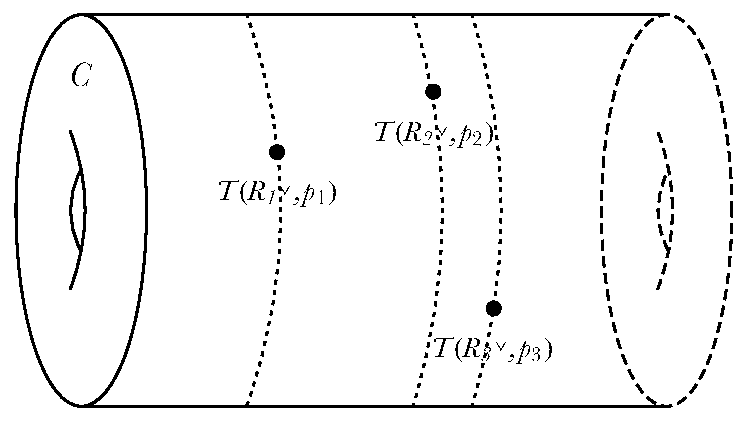
\includegraphics[scale=0.8]{Figures/Hooft}
	\caption{The insertion of three `t Hooft line operators into the 4D theory, corresponding to three point defects on the 3-manifold $W$. At each such insertion $p_i = (s_i, z_i)$, there will be a corresponding Hecke modification of a $G$-bundle over $C$ at the point $z_i$. Here the dashed lines denote the values $s_i \in I$ that the bundle undergoes a modification.}
	\label{fig:hooft1}
 \end{figure}
	
	 The only place where this is violated is at the values of $\sigma$ where the Bogomolny equations become singular. This is where we have the insertion of a monopole, corresponding to a `t Hooft modification of the bundle. This is exactly along the lines of the argument in Section~\ref{sub:from_the_yang_mills_higgs_action_on_mathbb_r_3}, where the insertion of a monopole at a radius $r$ away from the origin on $\rr^3$ modifies the holomorphic class of the bundle over $S^2_R$ as we go from $R < r$ to $R > r$. 
	 
	 
	 More generally, it is worth noting that this entire construction follows very closely the inverse scattering approach of Hitchin \cite{hitchin1982, atiyahhitchin1988}. In that case, the curve $C$ corresponded to the (non-compact) Riemann surface $\cc$ parameterizing the $x_1-x_2$ plane, and lines along the $x_3$ direction take the place of our $s$ variable along the unit interval $I$.
	
	\subsection{The Affine Grassmannian}

	In this section we make a mathematical detour to study the idea of Hecke modifications, which characterize the action of the `t Hooft operators on the holomorphic bundles over $C$ in our theory.
	
	\begin{defn}[Hecke Modification]
		Let $G$ be connected semisimple \footnote{Note that we will require $G$ to be both connected and semisimple, as otherwise the following logic would not work, even for $G=U(1)$.}. Given an associated $G$-bundle $E$ over a Riemann surface $C$, a \textbf{Hecke modification} of $E$ is a point $p \in C$ together with a choice of trivialization of $E$ on $C \backslash \{p \}$.
	\end{defn}
	
	
	\begin{obs}\label{obs:hecke}
			The Langlands dual is defined to have the property that any highest weight representation $\hat \rho: \hat G \to U(1)$ is dual to a morphism $\rho: U(1) \to G$ which can be viewed as a \emph{clutching function} for a $G$ bundle on the Riemann sphere $\mathbb{CP}^1$. Complexifying this gives $\rho: G_{\cc} \to \cc^\times \cong \mathbb{CP}^1 \backslash \{p, q \}$, AKA gluing a trivial bundle over $\mathbb{CP}^1 \backslash \{p \}$ to a trivial bundle over $\mathbb{CP}^1 \backslash \{q \}$. This is exactly what we call a Hecke modification of type $\rho$. Every holomorphic $G_{\cc}$-bundle over $\mathbb{CP}^1$ arises in this way.
	\end{obs}

	
	
	For our case, over $\mathbb{CP}^1$, Hecke modifications correspond exactly to a clutching function $\rho: \cc^\times \to G_\cc$ coming from a representation of the Langlands dual group. Following the convention of \cite{witten2010}, we write $\mathcal N(\rho)$ to denote the space of Hecke modifications of type $\rho$ over $\mathbb{CP}^1$.
	
	We now give some motivation for the next concept we will consider, namely the \textbf{affine Grassmannian}. The idea for this motivation was first introduced to the author in \cite{Yoo17}.
	\begin{mot}
		Consider a Hecke modification over a Riemann surface $C$. Since $C$ is a genus $g$ surface for some $g$, removing a point gives us a space equivalent to the punctured $2g$-gon, homotopically equivalent to a wedge of $2g$ circles. 
	
		Using the language of classifying spaces, the space of $G$ bundles over $C \backslash \{p\}$ is the homotopy classes of maps $\bigvee_{i=1}^{2g} S^1 \to BG$, which is captured by simply looking at $S^1 \to BG$, namely $\pi_1(BG)$. On the other hand, this is the same as $\pi_0(G)$, which is trivial for $G$ connected. Thus, we can find a trivialization on $C \backslash \{ p \}$. Similarly, around $p$ we have a disk $\mathbb D$ on which we can also find a trivialization.
		
		A gauge choice on a trivial bundle over a space $M$ is just a map $M \to G$. In our case we have three spaces: the disk $\mathbb D$, the punctured surface which we will denote $C^\times$, and the punctured disk $\mathbb D^\times$. 
		
		Then we have following three spaces of functions:
		\begin{itemize}
			\item $L_{in} = \mathrm{Map}(\mathbb D \to G)$, the gauge choices on $\mathbb D^\times$
			\item $L_{clutch} = \mathrm{Map}(\mathbb D^\times \to G)$, the clutching function
			\item $L_{out} = \mathrm{Map}(C^\times \to G)$, the gauge choices on $C^\times$.
		\end{itemize}
		
		Then a $G$-bundle on $C$ is specified by a clutching function modulo gauge transformations on both sides.
		Heuristically, then, in this picture we have
		\[
			\mathrm{Bun_G}(C) = L_{out} \backslash L_{clutch} / L_{in}.
		\]
	\end{mot}
	Letting $z$ be a local coordinate $C$ at $p$, the space of local gauge transformations in a formal neighborhood of $z$ can be viewed as formal power series in $z$ with values in the gauge group $G$. This is $G[[z]]$. For a linear algebraic group inside $\GL_n$, this can be viewed as $n\times n$ matrices with entries that are formal power series
	\[
		M = \begin{pmatrix}
			P_{11}(z) & \dots & P_{1n}(z)\\
			\vdots & \ddots & \vdots\\
			P_{n1}(z) & \dots & P_{nn}(z)\\
		\end{pmatrix}
	\]
	with the power series $P_{ij}(z) \in \cc[[z]]$ constrained so that $M \in G$. This captures the gauge transformations on $\mathbb D$. For the punctured disk, on the other hand, we are allowed to perform more general formal Laurent series, and so for us the corresponding ring (defined analogously) will be $G((z))$. 
	
	
	Given a trivialization on $C^\times$, the space of possible Hecke modifications at $p$ is exactly the space of clutching functions modulo gauge:
	\[
		L_{clutch} / L_{in} = G((z))/G[[z]].
	\]
	
	This is the motivation for our next definition.
	\begin{defn}[Affine Grassmannian]
		The affine Grassmannian $Gr_G$ of a semisimple group $G$ is the quotient space:
		\[
			Gr_G := G((z))/G[[z]].
		\]
	\end{defn}
	\noindent We state the following fact. For a more thorough intro, the reader is invited to see the notes of \cite{zhu2016}.
	\begin{fact}
		The Affine Grassmannian has a stratification into disjoint cells:
		\begin{equation}
			Gr_G = \bigsqcup_{\rho \in X_+(T)} \mathcal N(\rho)
		\end{equation}
		where $X_+$ are the dominant integral coweights of $G$ given maximal torus $T$. These correspond to the dominant integral weights of $\hat G$, are in canonical bijection with $\mathrm{Rep}(\check G)$.
	\end{fact}
	
	The affine Grassmannian plays an important role in the geometric Langlands correspondence. In particular, there is the \textbf{geometric Satake equivalence}, which states:
	\begin{theorem}[Geometric Satake]
		The ring of $G[[z]]$-invariant\footnote{With $G[[z]]$ acting by left multiplication} functions on $Gr_G$ is equivalent to the Grothendieck ring of representations of $\mathrm{Rep}(\check G)$.
	\end{theorem}
	In its original context \cite{satake1963} this relates the spherical Hecke algebras from Chapter~\ref{ch:intro} to the representation ring of $\check G$.
		
	\subsection{The Space of Hecke Modifications in the Physical Theory}
	
	We now conclude this thesis by connecting the `t Hooft operator picture to the picture of the affine Grassmannian. We consider a trivial bundle on $C$ and study how Hecke modifications act on it. In our picture of $W = I \times C$, we begin with Dirichlet boundary conditions at one end of $I$ and end with Neumann boundary conditions on the other end. We allow for `t Hooft operators to be inserted on $W$. In particular we denote a `t Hooft operator by two sets of data: the point $p_i$ where it is inserted and the representation $\check R_i$ of $\check G$ that corresponds to its type. The solutions to the Bogomolny equations of motion on $W$ are then exactly the space of Hecke modifications with these prescribed singularities.
	
	We denote this space by $\mathcal Z(\check R_1, p_1, \dots, \check R_k, p_k)$. This space is generically singular (10.3 of \cite{kapustin2006}). In order to be able to understand this space of solutions more clearly, we make use of the TQFT picture. The insertion of a `t Hooft operator of type $\check R$ at a point $p$ is equivalent to carving out a 2-sphere around $p$, $S^2_p$, and demanding that the vector bundle $E$ restricted to $S^2$ is obtained from a clutching function corresponding to $\check R$ (see Observation \ref{obs:hecke}).
	
	\begin{figure}[h]
		\centering
		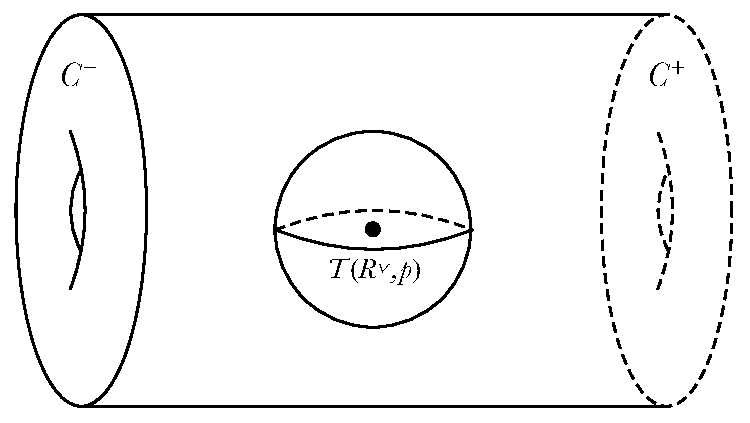
\includegraphics[scale=0.8]{Figures/Hooft2}
		\caption{An illustration of how the insertion of a `t Hooft operator of type $\check R$ equivalently gives rise to a cobordism $C^- \sqcup \mathbb{CP}^1 \to C^+$ with boundary conditions on $S^2$ arising from the $G$-bundle on $\mathbb{CP}^1$ induced by $\check R$.}
		\label{fig:hooft2}
	\end{figure}
	
	The classification of Hecke operators is thus very closely connected to the classification of $G$-bundles over $\mathbb{CP}^1$. 
	Working in the picture of Figure~\ref{fig:hooft2}, by viewing the insertion of a `t Hooft operator as a cobordism $C^- \sqcup \mathbb{CP}^1$ we see that $\mathcal Z(\check R_1, p_1, \dots, \check R_k, p_k)$ should have no explicit dependence on any of the points $p_i$. We will hence denote it just by $\ZZ(\check R_1, \dots, \check R_k)$.
	
	Though we will not prove this here\footnote{See sections 9 and 10 of \cite{kapustin2006} for a more detailed study of the space of solutions}, the space $\ZZ(\check R_1, \dots, \check R_k)$ factorizes . From the perspective of TQFT, this should be believable. If the insertion of a `t Hooft operator can be viewed as modifying the cobordism from $C^- \to C^+$ with prescribed boundary conditions into a cobordism from $C^- \sqcup \mathbb{CP}^1 \to C^+$, then the insertion of multiple `t Hooft operators gives
	\[
		C^- \sqcup \mathbb{CP}^1_1 \sqcup \dots \sqcup \mathbb{CP}^1_k \to C^+.
	\]
	By the locality axiom of TQFT, the category of boundary conditions associated to the disjoint union of $\mathbb{CP}^1_i$ should be some form of product of the categories associated to each individual $\mathbb{CP}^1_i$. The information about this category is contained in the solution space to the Bogomolny equations on $W$ so naively we would expect 
	\[
		\ZZ(\check R_1, \dots, \check R_k) = \prod_{i} \ZZ(\check R_i).
	\]
	This turns out to hold true.
	
	Now note
		$\ZZ(\check R)$ can be identified with the space of Hecke modifications of type $\check R$. If $\rho$ is the associated map $\rho: U(1) \to G$, then we can identify $\ZZ(\check R)$ with the Schubert cell $\mathcal N(\rho)$. 
	
	Both of these spaces are not compact, but have natural compactifications $\overline \ZZ(\check R), \overline{\mathcal N(\rho)}$. $\overline {\mathcal N(\rho)}$ will include Schubert cells associated to different representations of $\check G$. These will be exactly the representations with weights ``smaller'' than $\rho$ \cite{witten2010}. Physically this compactification has an interpretation in terms of the phenomenon of \textbf{instanton/monopole bubbling} and can be thought of in terms of collisions of the points $p_i$, c.f. section 10.2 of \cite{kapustin2006}.
	
	As we noted before, in a TQFT we should associate to each codimension 1 manifold a vector space of states. This means that (in the 4D theory) the space $W$ modified by the prescribed singularities $\{(p_i, \check R_i) \}$ has an associated vector space in the twisted $\mathcal N=4$ theory. How can we obtain such a space of states from $\overline{\ZZ}(\check R_1, \dots, \check R_k)$. The natural operation \cite{witten2010} is to take the cohomology of this space. To be more specific, because $\bar \ZZ$ is singular generically, the cohomology theory here will in fact correspond to the $L^2$ or \textbf{intersection cohomology}. From the side of mathematics, this has connections to perverse sheaves on the space, but we will not discuss that here. We thus define our Hilbert space to be
	\[
		\mathcal H(\check R_1, \dots \check R_k) := H^\bullet (\overline{\ZZ}(\check R_1, \dots, \check R_k)).
	\]
	
	By using the fact that \emph{the product of cohomologies is the cohomology of the product} we obtain the desired symmetric monoidal structure mirroring that of $\mathrm{Rep} (\check G)$:
	\begin{equation}
		\mathcal H(\check R_1, \dots \check R_k) = \bigotimes_{i=1}^k \mathcal H(\check R_i).
	\end{equation}
	
	Just as $\check R_i$ combine together to form tensors of irreducible representations, we see that the Hilbert spaces $\mathcal H(\check R_i)$ can be tensored together in the same way, corresponding to combining the classes of `t Hooft operators into a joint set of singularities on $W$. Thus, from the side of physics, we see an equivalence 
	\begin{equation}
		H^\bullet (Gr_G) \leftrightarrow \mathrm{Rep}(\check G).
	\end{equation}
	This is a variant of the geometric Satake equivalence. Moreover, this is the isomorphism of Tannakian categories studied by Deligne and Milne in \cite{deligne1982}.
	
	Given more time, I would have liked to extend this thesis to understand the action of `t Hooft operators on the categories of 2D boundary conditions in the twisted 4D theory.
	
	\newpage
	\begin{center}
		\emph{fin.}
	\end{center}
	
	% This suggests that there is an isomorphism of $\check R_i$ and $\mathcal H(\check R_i)$ as vector spaces. Indeed, it can be shown that such an isomorphism is the only way for these categories of (finite dimensional) vector spaces to have the same monoidal structure.
	
	% \section{A Final Note on Boundary Conditions} % (fold)
	% \label{sec:a_final_note_on_boundary_conditions}
	
	% section a_final_note_on_boundary_conditions (end)
	
	% \section{The Action of Wilson Loops on Boundary Conditions}
%
% 	\textbf{NOT FINISHED}
%
% 	If we assume that $M = \Sigma \times C$ for $C$ a compact Riemann surface and $\Sigma$ a (not necessarily compact) surface with boundary, we can study loop insertions more naturally. The following is a simplified picture of the general case:
%
% 	\begin{defn}[Hitchin's Moduli Space]
% 		$\mathcal M_H (G, C)$ is the space of solutions to the Hitchin equations on a curve $C$.
% 	\end{defn}
% 	If we consider $C$ to be ``small'' relative to $\Sigma$, for each point in $\Sigma$, the additional data for the field configurations on the space $C$ must give us a point in this moduli space. That is, we get a nonlinear sigma model on $\Sigma \to \mathcal M (G, C)$.
%
% 	Let the curve defining a (Wilson or `t Hooft) operator be $\gamma = \gamma_0 \times p$ in $\Sigma \times C$ with $p$ a point on $C$ and $\gamma_0$ a curve on $\Sigma$. Let $\partial \Sigma_0$ be a connected component of $\partial \Sigma$. A boundary condition for the field theory on $\Sigma_0$ is called a \textbf{brane}.
%
% 	Let $\gamma_0$ approach this boundary. On the $\hat B$ side, the insertion of a Wilson loop acts as an associative endofunctor for the category of boundary conditions on the topological sigma model on $\Sigma$ with target $\mathcal M_H (G, C)$. This target  space, with choice of complex structure $J$, can be identified with $\mathcal M_{flat} (G, C)$.
%
% 	\begin{figure}
% 		\centering
% 		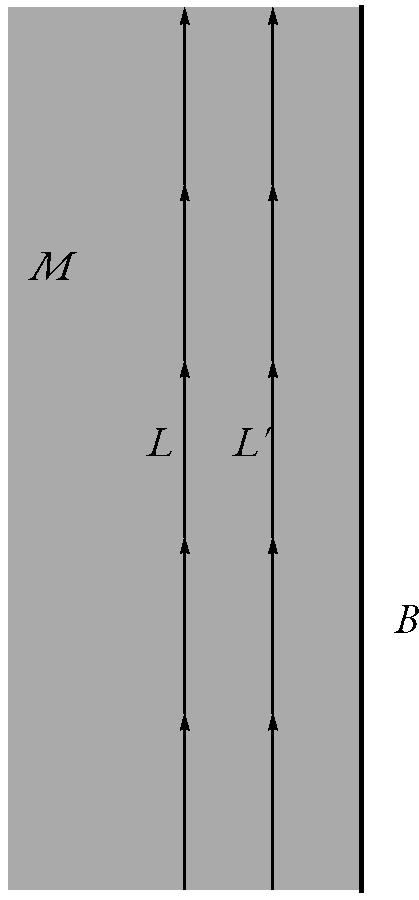
\includegraphics[scale=0.5]{figures/Wilson}
% 		\caption{The insertion of two Wilson lines approaching a boundary. They act associatively on the category of boundary conditions, and have actions commuting with one another.}
% 		\label{fig:wilson}
% 	\end{figure}
%
% 	 This functor will depend on the point $p \in C$ corresponding to the Wilson line. Consider the product $\mathcal M_{flat} (G, C) \times C$. There is a universal $G$-bundle $\mathcal E$ over this space, given by taking a point in $\mathcal M_{flat}$ and restricting the corresponding bundle to a point in $C$.
%
% 	Given any coherent sheaf on $\mathcal M_{flat}$, we can tensor this with $R(\mathcal E)$. This is the action of the Wilson loop insertion on the space.
%
% 	Consider the structure sheaf $\mathcal O_x$ of a point $x \in \mathcal M_{flat}(\check G, C)$. For any representation $\check R$, the Wilson loop maps $\mathcal O_x$ to $\mathcal O_x \otimes \check{R}$.
% 	Thus $\mathcal O_x$ is an eigen-object for the functor $W_{\check R}(p)$, which acts on it by tensoring it with the vector space $\check R(\mathcal E_p)_x$. In fact, letting $p$ vary we see that it is an eigen-object for all $W_{\check R}(p)$. Another way of saying this is that the eigenvalue is the flat $\check G$-bundle $\check R(\mathcal E)_x$ on $C$.
%
% 	More directly, this flat bundle is obtained by taking the flat principle bundle on $C$ corresponding to $x$ and forming the associated bundle via $\check R$.
%
% 	The action of the `t Hooft operators is more difficult to see. They will end up acting by Hecke transformations on the space of boundary conditions. By Monotonen-Olive duality, it turns out that the brane corresponding to a fiber of the Hitchin fibration in $\mathcal M_H(G, C)$ is a common eigenobject for all operators.
%
